\chapter{Naive Bayes}

\section{Pré-traitement des données}

Nous avons d'abord effectué un pré-traitement des données en utilisant différentes techniques :

\subsection{Tokenisation des commentaires}

Nous avons utilisé la tokenisation pour diviser les commentaires en tokens individuels.

\subsubsection*{Tokenisation à l'aide de nôtre API \texttt{tokenize\_apy}}

La tokenisation des commentaires a été réalisée en utilisant l'API \texttt{tokenize\_apy}.

\subsubsection*{Équilibrage du jeu de données}

Nous avons équilibré le jeu de données en échantillonnant un nombre égal de commentaires toxiques et non toxiques.

\section{Analyse exploratoire des données}

Voici les statistiques descriptives sur le jeu de données équilibré :

\subsection{Statistiques descriptives}

\begin{itemize}
    \item Nombre total de documents : 25 962
    \item Nombre total de tokens : 127 656
    \item Nombre de classes à prédire : 2 (toxique ou non toxique)
    \item Les tokens les plus fréquents incluent "grand", "ter", "burn", etc.
\end{itemize}

\section{Entraînement du modèle}

Nous avons entraîné le modèle Bayésien naïf en suivant les étapes suivantes :

\subsection{Préparation des données}

\begin{itemize}
    \item Calcul de la fréquence des mots et sélection des stop words.
    \item Entraînement du modèle en utilisant \texttt{CountVectorizer} et \texttt{MultinomialNB}.
\end{itemize}

\subsection{Évaluation des performances du modèle}

\begin{table}[h]
    \centering
    \begin{tabular}{|l|l|l|l|l|l|l|l|}
    \hline
    \textbf{Technique de prétraitement} & \textbf{Précision} & \textbf{Rappel} & \textbf{F1-score} & \textbf{Support} \\ \hline
    comment\_text\_word\_tokenize\_no\_normalization & \textbf{0.89} & \textbf{0.89} & \textbf{0.89} & 5193 \\ \hline
    comment\_text\_gpt\_tokenize\_no\_normalization & \textbf{0.89} & \textbf{0.89} & \textbf{0.89} & 5193 \\ \hline
    comment\_text\_word\_tokenize\_normalization & 0.87 & 0.87 & 0.87 & 5193 \\ \hline
    comment\_text\_gpt\_tokenize\_normalization & 0.87 & 0.87 & 0.87 & 5193 \\ \hline
    comment\_text\_word\_tokenize\_full\_normalization & 0.87 & 0.87 & 0.87 & 5193 \\ \hline
    comment\_text\_gpt\_tokenize\_full\_normalization & 0.87 & 0.87 & 0.87 & 5193 \\ \hline
    comment\_text\_word\_tokenize\_simple\_normalization & 0.88 & 0.88 & 0.88 & 5193 \\ \hline
    comment\_text\_gpt\_tokenize\_simple\_normalization & 0.88 & 0.88 & 0.88 & 5193 \\ \hline
    \end{tabular}
    \caption{Performances du modèle Bayésien naïf avec différentes techniques de prétraitement}
\end{table}

\subsection{Validation croisée}

Nous avons également effectué une validation croisée en utilisant la métrique \texttt{f1\_macro}.

\begin{table}[h]
    \centering
    \begin{tabular}{|l|l|}
    \hline
    \textbf{Métrique} & \textbf{Score} \\ \hline
    f1\_macro (moyenne) & 0.888 \\ \hline
    f1\_macro (écart type) & 0.004 \\ \hline
    \end{tabular}
    \caption{Résultats de la validation croisée}
\end{table}

\section{Analyse des résultats}

\subsection{Calcul des probabilités}

\begin{itemize}
    \item Probabilités a priori pour chaque classe : \{0: 0.501, 1: 0.499\}
    \item Vocabulaire contient 46 849 mots uniques
\end{itemize}

\subsection{Calcul des vraisemblances}

Nous avons calculé les probabilités conditionnelles (vraisemblances) pour chaque mot dans chaque classe.

\subsection{Prédiction}

Nous avons utilisé le modèle entraîné pour prédire la toxicité des commentaires de test. Par exemple, le commentaire "chretian attack" a été prédit comme toxique avec une probabilité de 0.000168.

\subsection{Matrice de confusion}

La matrice de confusion montre que le modèle prédit correctement les commentaires toxiques et non toxiques dans une large mesure.

\begin{figure}[h]
    \centering
    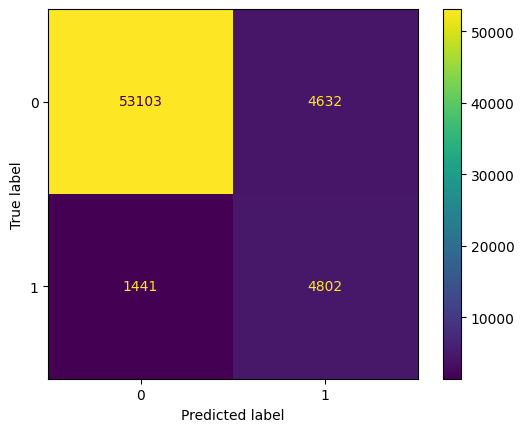
\includegraphics[width=.49\linewidth]{figures/matrix-confusion-naive_bayes.png}
    \caption{Matrice de confusion du modèle Bayésien naïf}
\end{figure}

\subsection{Fonction de prédiction}

Nous avons également créé une fonction \texttt{isToxicity} qui prend en entrée un commentaire et prédit sa toxicité.

\subsection{Distribution de la toxicité globale}

\begin{figure}[h]
    \centering
    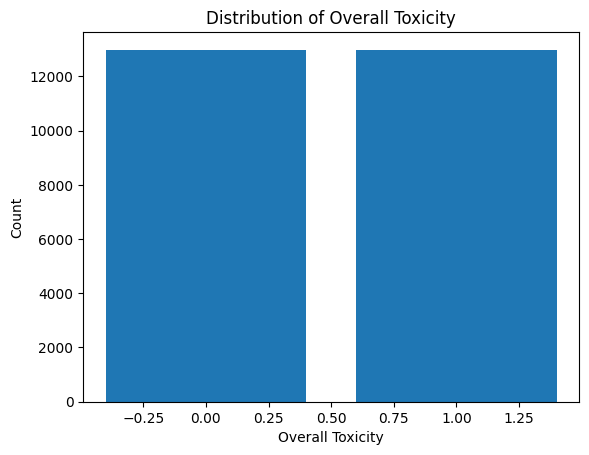
\includegraphics[width=.47\linewidth]{figures/distribution-toxicity-naive_bayes.png}
    \caption{Distribution de la toxicité des commentaires}
\end{figure}

\end{document}
